\section{Proposed Method}
\label{sec:proposed_method}

The method hereby presented is based on the idea of approximating the probability distribution of a set of solutions using an energy-based model. In particular, we exploit the remarkable approximation capabilities of neural networks to estimate the fitness of a solution set. By also treating the neural network as an energy-based model, we can then equate the fitness of a solution to the energy computed by the model\footnote{In this work, we want to minimise the fitness function rather than maximise it as it was done in the original DEUM paper.}. Then, to minimise the Kullback-Leibler divergence between the empirical distribution of the population and the model, we can simply train the model by minimizing the Mean Squared Error (MSE) between the predicted energy and the actual fitness of the population. Furthermore, we can easily sample from the model using Langevin dynamics.

Hereafter, we will describe the two main components of the proposed method: the energy-based model and the local sampling. The energy-based model can be further divided into three sub-components: gene embeddings, structure learning and energy regressor.

\begin{figure}[H]
    \centering
    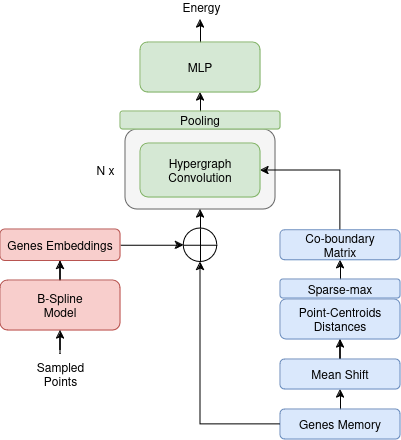
\includegraphics[width=0.35\textwidth]{img/model.png}
    \caption{Proposed architecture}
    \label{fig:method}
\end{figure}

\subsection*{Gene Embeddings}

As stated above, the energy-based model is used to predict the fitness of a solution $\mathbf{x} \in \mathbb{R}^n$ represented as a vector of $n$ genes. While it would be possible to directly use the genes values as input to the model, it has been shown in many domains that neural networks can benefit from transforming floating point values into vectorial representations.

As Langevin dynamics requires to compute the gradient of the energy with respect to the input, traditional encodings, like sinusoidal or gamma encodings, would not be suitable as they multiply the input by an exponential function, making the gradient too large. For this reason, we propose to use learnable B-spline functions to map each gene value to a higher-dimensional space. In particular this mapping is done as a weighted summation:
\begin{equation*}
    \mathbf{g}(\mathbf{x}_j) = \sum_{i=0}^n \mathbf{p}_i N_{i,m}(\mathbf{x}_j)
\end{equation*}
where $\mathbf{x}_j$ is the j-th gene, $\mathbf{p}_j$ are the learnable n-dimensional control points and $N_{i,m}$ are B-spline functions.

A B-spline of order $m+1$ is a series of piece-wise polynomial functions $N_{i,m}(t)$ of degree $m$. The points $T=t_0, t_1, \dots, t_m$, where these polynomials intersect, are known as knots and are typically placed equidistantly. A B-spline is recursively defined as follows:
\begin{align*}
    N_{i,0}(t) & = \begin{cases}
                       1 & \text{if } t_i \leq t < t_{i+1} \\
                       0 & \text{otherwise}
                   \end{cases}                                                                   \\
    N_{i,m}(t) & = \frac{t - t_i}{t_{i+m} - t_i} N_{i,m-1}(t) + \frac{t_{i+m+1} - t}{t_{i+m+1} - t_{i+1}} N_{i+1,m-1}(t)
\end{align*}
\subsection*{Structure Learning}

Following the idea of multivariate EDAs, we aim to learn the dependencies between genes to better model the fitness landscape for those problems where the genes exhibit epistasis. To do so, we view each gene as a node in a graph and we learn to cluster genes that exhibit high dependencies, thus effectively moving from a graph to a hypergraph representation.

To learn the hypergraph structure, we associate to each gene a learnable memory vector $\mathbf{m}_i \in \mathbb{R}^d$ that should encode the gene's role in the problem structure. The idea is that during the training process, genes that are dependent on each other will be pushed closer in the embedding space and thus will be clustered together.

To do so, we use mean-shift on the genes memories to compute the cluster centroids $\mathbf{C} \in \mathbb{R}^{k \times d}$, where $k$ is the number of clusters found. We then compute the cosine distance between the genes' memories and the returned centroids, obtaining a soft membership matrix that we row-wise normalize to 1. While multiple normalization functions could be used (simple summation, softmax, etc.), we choose to use the entmax-2 function \cite{martins_sparsemax_2016} as it guarantees sparsity in the output.

The resulting normalized matrix can then be considered the co-boundary matrix of the hypergraph $\mathbf{B} \in \mathbb{R}^{n \times k}$, indicating for each gene the hyperedges it belongs to.

\subsection*{Energy Regressor}

The energy regressor uses the gene embeddings and the hypergraph structure to estimates the fitness of the input individual.

Here we take a different approach from traditional undirected graphical models. In these models, the energy of a configuration is computed as the sum of the potential functions, where each potential function is defined only over the nodes of the corresponding clique. Thus, there is no direct interaction between the nodes of different cliques or between cliques themselves. Opposite to this approach, we believe that the fitness of a solution is also influenced by the interactions between groups of genes, and not only by the interactions within each group. For this reason, we propose to stack multiple hypergraph convolutional layers \cite{bai_hypergraph_2019} to allow each node to exchange information with all the other nodes in the hypergraph while still preserving the hypergraph structure.

In particular, the embeddings given in input to the first layer are computed as the sum of the gene embeddings and the gene memories that serve as a sort of positional embeddings, i.e. $\mathbf{Z}^0 = \mathbf{E} + \mathbf{M}$. Then, the embeddings are passed through multiple hypergraph convolutional layers, where the output of the $l$-th layer is computed as:

\begin{equation*}
    \mathbf{Z}^{l} = \sigma(\mathbf{B}\mathbf{B}^\intercal \mathbf{Z}^{l-1} \mathbf{W}^{l})
\end{equation*}

where $\sigma$ is the activation function and $\mathbf{W}^{l}$ is the weight matrix of the $l$-th layer.

The embedding of the input solution is then obtained by applying a permutation-invariant pooling function to the output of the last layer. In this work, we use mean-pooling, but other pooling functions could be used as well. To compute the final energy of the solution, the pooled embeddings are passed through a multi-layer perceptron (MLP) with a single output neuron:

\begin{equation*}
    E(x) = \text{MLP}(\text{pool}(\mathbf{Z}^{L}))
\end{equation*}

\subsection*{Local Sampling}

As the energy-based model is trained to approximate the fitness landscape, sampling from it can be used to obtain the more promising solutions as they have lower energy and thus higher probability. However, we found that simply applying Langevin dynamics to the model can lead to poor results. Indeed, if the fitness landscape is multimodal or very smooth, million of samples are needed to find the global optima.

To address this issue, we propose to use a modified version of Langevin dynamics that uses an adaptive noise parameter (instead of a static one) $\eta$:

\begin{equation*}
    x_{t+1} = x_t - \epsilon \nabla E(x_t) + \eta \cdot \mathcal{N}(0, I)
\end{equation*}

that can be used to bias the sampling process to stay within a region centered aroung the starting point $x_0$.

At each iteration of the optimization process, we sample a new batch of points using Langevin dynamics and the points generated in the previous iteration as starting points. We then cluster the generated points using mean-shift and we consider the clusters centroids as the basins of attraction around which we generate new points. In particular, the generation is performed by sampling from a multivariate normal distribution whose parameters are fitted on the cluster's points. Furthermore, to focus the exploration on the more promising areas of the search space, we generate for each cluster a number of points inversely proportional to the average energy of its original points.

Finally, we adjust the noise size of each cluster based on a base noise $\lambda$, the cluster extension $\delta$ and how much the cluster fitness has improved from the previous iteration:

\begin{align*}
    \delta(C_{i,t}) & = \max_{i} x_i - \min_{i} x_i \forall x \in C_{i,t}                                                                        \\
    \phi(C_{i,t})   & = \begin{cases}
                            \sqrt{f(C_{i,t}) / f(C_{i, t-1}) } & \text{if } \exists C_{i, t-1} \sim C_{j,t} \\
                            1                                  & \text{otherwise}                           \\
                        \end{cases} \\
    \eta_i          & = \lambda \delta(C_{i,t}) \phi(C_{i,t})
\end{align*}

To determine whether the fitness of a cluster has improved, we need to match the clusters from the current iteration to the clusters from the previous iteration. To do so, we compute the inter-cluster distance between each pair of new and old clusters. If no distance is below a certain threshold, the cluster is considered new, otherwise, it is matched to the closest cluster.

The adaptive noise parameter is a form of trade-off between exploration and exploitation: if the cluster has improved and became more compact, the noise is reduced, allowing the search to focus on the found optima. On the other hand, if the cluster has not improved or has expanded, the noise is increased, incentivizing exploration of different areas.

\begin{figure}
    \centering
    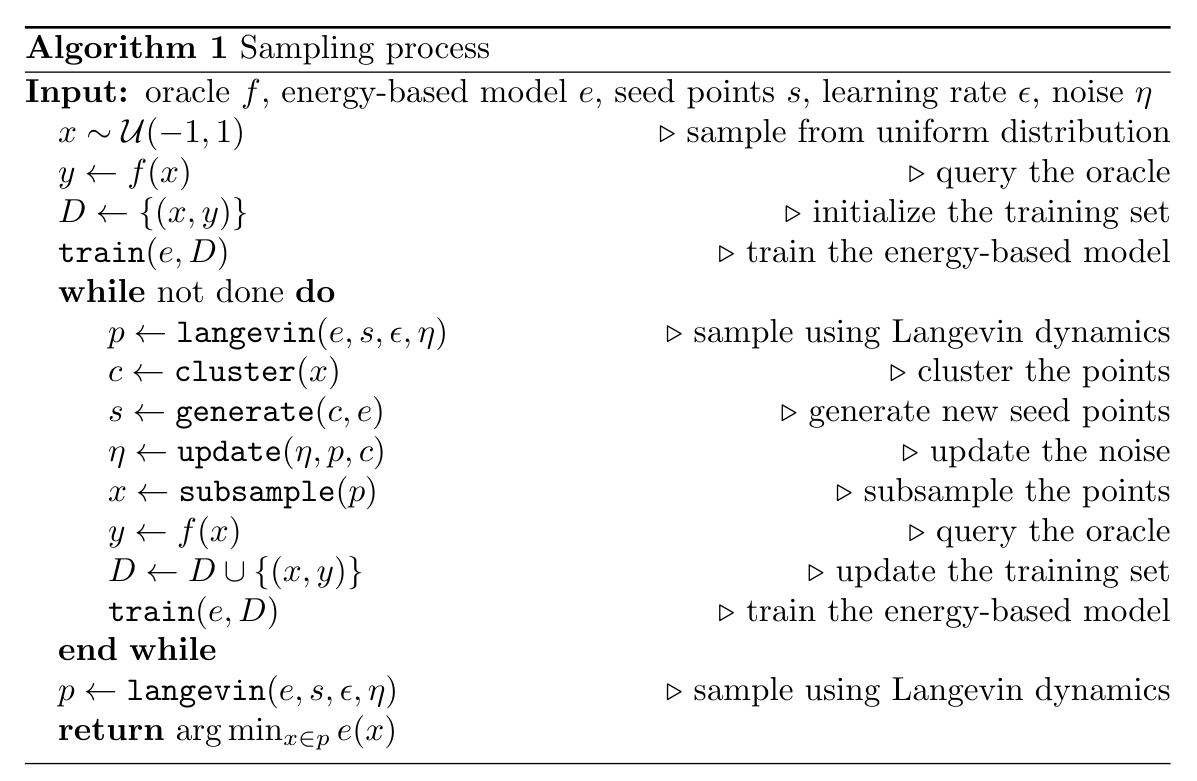
\includegraphics[width=\columnwidth]{img/sampling.png}
    \caption{Sampling process}
    \label{alg:sampling}
\end{figure}

From the algorithm above (see Figure \ref{alg:sampling}), one can see that differently from EDAs, the new parameters of the model are not fitted only on the new best sampled points, but on the whole history of the sampling process. This is necessary as neural networks suffer from catastrophic forgetting and poor out-of-distribution generalization. If we were to train the model only on the new points, it may start assigning low energy to the old points, thus making the search go back to the same regions.
